% Daniel Schurholz, modified version from Jouni Ritvanen's doctoral version
%
% Compile to pdf, run at command prompt:
% latex main
% makeindex main.nlo -s nomencl.ist -o main.nls
% bibtex main
% latex main
% latex main
% dvipdfm main.dvi

\documentclass[a4paper,twoside,12pt,notitlepage,openright]{article}
\usepackage[ansinew]{inputenc}
\usepackage{graphicx} %[dvips] to used with .eps figures
\usepackage{natbib}
\usepackage{lastpage}   % page count
\usepackage{amsmath}
\usepackage{amssymb}
\usepackage[english]{babel}
\usepackage[intoc]{nomencl} % including table of content
\usepackage{ifthen}
\usepackage[hmargin=3.0cm,vmargin=3.6cm]{geometry} % setting marginals
\usepackage{fancyhdr}  % header ja footer manipulation
\usepackage{times}  % to change font to times
\usepackage{setspace} % for linespacing
\usepackage{xstring}
\usepackage{tabularx}
\usepackage{etoolbox}

\pretocmd{\chapter}{\addtocounter{totfigures}{\value{figure}}\setcounter{figure}{0}}{}{}
\pretocmd{\chapter}{\addtocounter{tottables}{\value{table}}\setcounter{table}{0}}{}{}

\newcolumntype{Y}{>{\centering\arraybackslash}X}

\newcommand{\nomunit}[1]{\renewcommand{\nomentryend}{\hspace*{\fill}#1}} % Inserts units on the right at symbol list
\renewcommand{\nomgroup}[1]{%
 \ifthenelse{\equal{#1}{C}}{\item[\textbf{Latin alphabet}]\item}{%
 \ifthenelse{\equal{#1}{G}}{\item\item[\textbf{Greek alphabet}]\item}{}}{%
 \ifthenelse{\equal{#1}{L}}{\item\item[\textbf{Subscripts}]\item}{}}{%
 \ifthenelse{\equal{#1}{H}}{\item\item[\textbf{Superscripts}]\item}{}}{%
 \ifthenelse{\equal{#1}{W}}{\item\item[\textbf{Abbreviations}]\item}{}}{}}

\onehalfspacing

\pagestyle{fancy}

%% FANCY FOOTER
\fancyhf{}% clearing the header and footer
\renewcommand{\headrulewidth}{0pt}
\cfoot{\bfseries\thepage}
%%

%% FANCY HEADER
% For page number in header + section name, uncomment next 10 lines and comment previous 3 lines
% \fancyhf{}
% \fancyhead[LE,RO]{\bfseries\thepage}    % page number to header
% \fancyhead[LO]{\nouppercase{\bfseries\rightmark}}     %
% \fancyhead[RE]{\nouppercase{\bfseries\leftmark}}%
% \renewcommand\sectionmark[1]
%  {\markboth{\thesection\ #1}{}}         % section name to header
% \renewcommand\subsectionmark[1]
%  {\markright{\thesubsection\ #1}}       % subsection name to header
% \renewcommand{\headrulewidth}{0.5pt}    % ruler thickness between head and body
% \renewcommand{\footrulewidth}{0pt}      % no ruler between body and footer
%%

\setlength{\nomitemsep}{-\parsep}   % removing default extra skip between entries at nomenclature

\numberwithin{equation}{section}    % equation numbers with section numbers
\numberwithin{table}{section}       % table numbers with section numbers
\numberwithin{figure}{section}      % figure numbers with section numbers

% makeindex command needs to run at command prompt to create nomenclature list file
\makenomenclature % makeindex main.nlo -s nomencl.ist -o main.nls
%\bibpunct{(}{)}{;}{a}{,}{,}%
\AtBeginDocument{%
    \renewcommand\contentsname{TABLE OF CONTENTS}
    \renewcommand\nomname{LIST OF SYMBOLS AND ABBREVIATIONS}
    \renewcommand*\listfigurename{LIST OF FIGURES}
    \renewcommand*\listtablename{LIST OF TABLES}
}

\newcounter{totfigures}
\newcounter{tottables}

\providecommand\totfig{} 
\providecommand\tottab{}

\makeatletter
\AtEndDocument{%
  \addtocounter{totfigures}{\value{figure}}%
  \addtocounter{tottables}{\value{table}}%
  \immediate\write\@mainaux{%
    \string\gdef\string\totfig{\number\value{totfigures}}%
    \string\gdef\string\tottab{\number\value{tottables}}%
  }%
}
\makeatother

\pretocmd{\section}{\addtocounter{totfigures}{\value{figure}}\setcounter{figure}{0}}{}{}
\pretocmd{\section}{\addtocounter{tottables}{\value{table}}\setcounter{table}{0}}{}{}

\begin{document}

\pagestyle{empty}
\newcommand{\thesisAuthor}{Your Name}
\newcommand{\thesisTitle}{Your Thesis Title}

% The Participating Universities
\newcommand{\universities}{Universit\'{e} de Lorraine\\
Lappeenranta University of Technology\\
Lule\r{a} University of Technology\\}

% Your supervisors in the order that you want them printed, just add or remove lines and change the indexes if needed.
\newcommand{\supervisors}[1]{
    \IfEqCase{#1}{
        {0}{Supervisor 1}
        {1}{Supervisor 2}
        {2}{Supervisor 3}
    }[\PackageError{constants}{Undefined option to supervisors: #1}{}]%
}

% Your examiners in the order that you want them printed, just add or remove lines and change the indexes if needed.
\newcommand{\examiners}[1]{
    \IfEqCase{#1}{
        {0}{Prof. Eric Rondeau}
        {1}{Prof. Jari Porras}
        {2}{Prof. Karl Andersson}
    }[\PackageError{constants}{Undefined option to examiners: #1}{}]%
}

% Your keywords in the order that you want them printed, just add or remove lines and change the indexes if needed.
\newcommand{\keywords}[1]{
    \IfEqCase{#1}{
        {0}{this}
        {1}{are}
        {2}{very}
        {3}{awesome}
        {4}{keywords}
    }[\PackageError{constants}{Undefined option to keywords: #1}{}]%
}

\newcommand{\keywordList}[2]{
    \newcount\idx
    \newcount\lastEl
    \idx=0
    \lastEl=#1
    \advance \lastEl-1
    \loop
        \keywords{\the\idx}\ifnum \idx<\lastEl#2\fi
    \advance \idx+1
    \ifnum \idx<#1
    \repeat
}

\thispagestyle{empty} \setlength{\parindent}{0pt}
~\\

\large\universities
\vspace{40mm}

\large{\textbf{\thesisAuthor}}\\
\vspace{2mm}\\

\MakeUppercase{\Large{\textbf{\thesisTitle}}}\\
\vspace{40mm}

\begin{tabular}{@{}l p{11.0cm}}
Examiners:
&\examiners{0}\\
&\examiners{1}\\
&\examiners{2}\\
\\
Supervisors:
&\supervisors{0}\\
&\supervisors{1}\\
&\supervisors{2}\\
\end{tabular}

\pagebreak

\normalsize
\section*{ABSTRACT}

\universities
\\
\thesisAuthor\\
\\
\textbf{\thesisTitle}\\
\\
Master's Thesis\\
\\
\pageref{LastPage} pages, \totfig\ figures, \tottab\ tables, 1 appendix\\
\\
\begin{tabular}{@{}l p{11.0cm}}
Examiners:
&\examiners{0}\\
&\examiners{1}\\
&\examiners{2}\\
\end{tabular}\\
\\
Keywords: \keywordList{5}{,}.\\
\\
% Actual Abstract
\par{Lorem ipsum dolor sit amet, mei integre propriae in, dolorum explicari disputando et sit. Ius tractatos molestiae eu. Et agam utroque vel, illud veritus pro an, iudico ornatus volutpat eam no. Sit liber scribentur neglegentur in, et ignota regione impedit sit. Propriae postulant sed cu. Eam ad velit graeco accusam, denique elaboraret qui eu. Sit in adhuc fabulas admodum, recteque intellegebat eam an, eu pri movet aeterno. Est at dicat inani petentium, an simul fabellas mei. Pri impetus deterruisset te, ex paulo consulatu qui, nihil bonorum adolescens ad quo. Qui et evertitur dissentias, cum ei affert incorrupte. Ex possim discere alienum nam. Inani putant partiendo ea sit, in dolore eruditi vim, est unum verear ad. Quo nominati mediocrem molestiae eu. Nominati aliquando appellantur ad quo, solum inermis recteque ad nam, mollis definitionem his ut. Nec an diam accusam. Per et nullam ridens. An his solet tritani assueverit. Zril democritum at pri. Ea duo affert integre reprimique, idque putent honestatis eu vis. Solet dictas usu ex, saepe primis nostrum mea no. Ludus patrioque tincidunt est an, postea numquam interpretaris cum ne, qui ex duis semper intellegam.}

\addtocontents{toc}{\contentsline {section}{ABSTRACT}{}}

\section*{ACKNOWLEDGEMENTS}

The contents of this page are totally up to the author. Acknowledgements, mentioning
something about the laboratory/working place/key people furthering the work may be
mentioned. See the "Final thesis instructions" in the study guide.\\

Thanks.\\

\vspace{\stretch{1}}
Your name\\
March 2019\\
Skellefte\r{a}, Sweden\\

\addtocontents{toc}{\contentsline {section}{ACKNOWLEDGMENTS}{}}%
\addtocontents{toc}{\contentsline {section}{TABLE OF CONTENTS}{}}%
\addtocontents{toc}{\contentsline{section}{LIST OF FIGURES}{}}
\addtocontents{toc}{\contentsline{section}{LIST OF TABLES}{}}

\tableofcontents%
\thispagestyle{empty}%
\clearpage%
\listoffigures
\thispagestyle{empty}%
\clearpage%
\thispagestyle{empty}%
\listoftables
\thispagestyle{empty}%
\clearpage%
\pagestyle{fancy}%

\thispagestyle{empty}%
\cleardoublepage%
\printnomenclature[2.0cm]%

\setlength{\parskip}{\baselineskip}%
\section{INTRODUCTION}\label{sec:intro}

\subsection[BACKGROUND]{Background}
\par The goal of this report is to give instructions how to write a master's thesis. The report is only an outline, a model which will be extended according to the contents of the actual work for the thesis. For more information, read ``Final thesis instructions'' in the study guide, discuss with your supervisor, visit appropriate course web pages, see for example [1].  When you are referring to pages in the (WWW)\nomenclature[WWWW]{WWW}{World Wide Web}, see the instruction for citing and referencing from the LUT Library web site. Do not use footnotes or do not write URLs within the text. 

\par Introduction contains three subsections: background, goals and delimitations, and description of the structure of the thesis. Use this sectioning.  Subsection 1.1 includes an introduction to the background for the work.  Remember that the abstract is a separate piece of text. The introduction should be written independently such that one does not need to read the abstract to understand the introduction.  The introduction is written in a general level instead of many details present. These details will be explained later starting from section 2. The paragraphs have more than only one sentence. In the thesis, this subsection occupies from 1 to 2 pages.

\par Remember to introduce the abbreviations when they are used in the text for the first time. For example: ``This thesis is about the games played in National Hockey League (NHL)\nomenclature[WNHL]{NHL}{National Hockey League} in seasons 1900-2000. The annual penalties in NHL have ...''.

\par The introduction is written such that the reader is interested to continue to read the full thesis. And if this interest is arisen then the author is ready to give some general descriptions for the contents of the thesis and reading guidelines for the rest of the text in the thesis.

\clearpage

\subsection[GOALS AND DELIMITATIONS]{Goals and delimitations}

\par Express the goals for the work, include also the delimitations. This way the reader knows when the results are valid and she can place the work in a proper framework and scope. It is also important to say, what is not done during the work for the thesis. Then the thesis will show how the goals are met. In the thesis this subsection occupies from 1 to 2 pages.

\subsection[STRUCTURE OF THE THESIS]{Structure of the thesis}

\par This subsection contains a short description for the contents of the thesis. The contents of each section are characterized with one or two sentences. For example: ``Section 2 contains a description of the ...''. In the thesis this subsection occupies at most one page, in many cases half a page is enough. At this point, one should thoroughly consider the structure of work. Discuss with your supervisor about the structure.
\citep{Dur00}.
 %Introduction
\section{THESIS}\label{sec:thesis}

\subsection[TYPES OF MASTER'S THESIS]{Types of master's thesis}
\par Start each section from a new page. The second section normally contains a more detailed introduction to the topic. For example, this document might have an introduction to various types for master's thesis.

\subsection[CITING AND REFERENCES]{Citing and references}
\par{Include a cite in the text for all figures, tables, references, and appendices. There are no exceptions for this rule. Use increasing numbering in citing. Appendix 1 acts as an example for an appendix.}

\par{Citing can be as follows: ``In digital imaging contrast enhancement may lead into higher dynamics as shown in Fig. \ref{fig:figimage}.''  If the image is taken from some source, e.g. from a book, the source is mentioned in the caption.  The figure itself comes after the cite in the text, this means that the figure is mentioned in the text before the figure presented. The figure comes after the end of the paragraph. The alignment of the figure and the caption is centered. The caption is always under the figure. The heading of a table is above the table, an example is given in Table \ref{tab:table1}. Table \ref{tab:table1} is an example of a table. The table heading and the table itself are aligned in the center. The texts in the figure caption and in the table heading are closed with a period. The caption and the heading may contain several sentences.}

\begin{figure}[h]
\begin{tabular}{c c}
  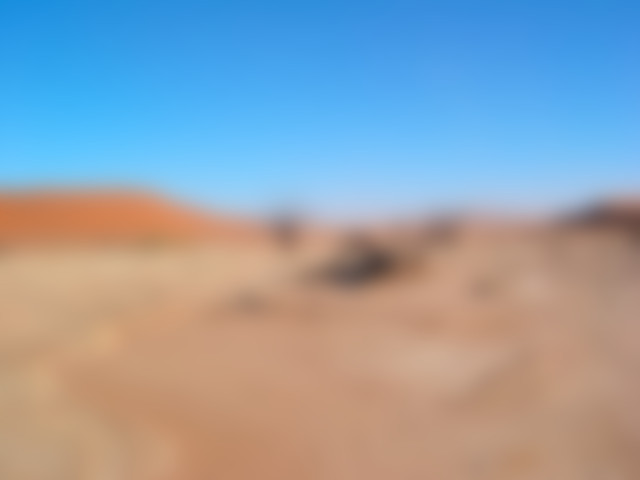
\includegraphics[width=0.45\textwidth]{./figs/image2.jpg} &
  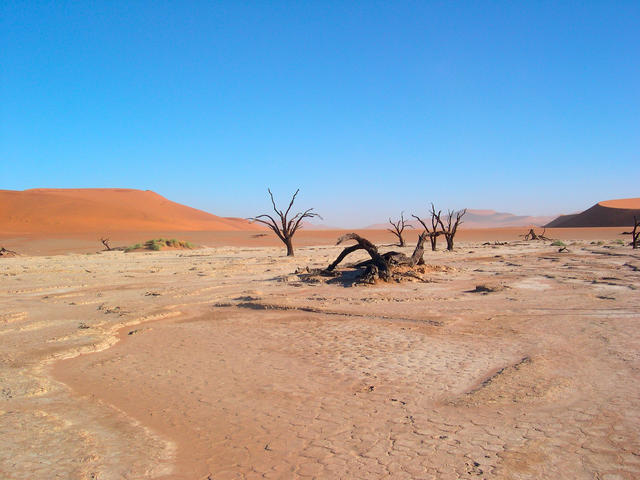
\includegraphics[width=0.45\textwidth]{./figs/image1.jpg}\\
  \hspace{1.2cm}(a) & \hspace{1.2cm}(b) \\
\end{tabular}
\caption[Contrast enhancement.]{Contrast enhancement: a) original image; b) enhanced image \citep{Ahm85}.} \label{fig:figimage}
\end{figure}

\par The figure with the caption and the table with the heading appear as full on one page, do not split them over several pages. For example, Fig. \ref{fig:figimage} and Table \ref{tab:table1} are on one page only. Figures and tables are placed such that there is no extra empty space above or below the image. Normally, figures and tables are placed on top of the page or on the bottom of the page, but they may appear also in the middle. If the figure or the table can not be placed on the same page as the paragraph with the cite then place the figure and the table on the next page. The bottom of the page is filled with the text from the next paragraph.

\begin{table}[h]
  \centering
  \caption[Grading]{Scaling for grading.} \label{tab:table1}
  \begin{tabularx}{0.8\textwidth}{| X | Y | Y | Y | Y |}
  \hline
  Points & 0-10 & 11-20 & 21-30 & 31-40 \\
  \hline
  Grades & 1 & 2 & 3 & 4 \\
  \hline
  \end{tabularx}
\end{table}

\par References are given in the list of references, either in alphabetical order or in citing order. The latter means that the references are listed exactly in the order they are cited in the text. The cites and the corresponding references are numbered as [2] or according to the first author with the year of the publication (K\"{a}lvi\"{a}inen, 2010). If there are several authors, the form for citing is (K\"{a}lvi\"{a}inen, et al., 2008).  All references contain full bibliographic information such that the article can be unambiguously identified. An example for a scientific article [3] and a conference article [4] are here. There is never a cite at the end of a chapter, outside all sentences, i.e. no cite after the dot after the last sentence of a paragraph. The author should always express clearly what comes from a reference and what is produced by the author. 

\par Equations are always numbered and they are part of the text. The presentation is not disconnected because of an equation. Here is an example how to include an equation in the text:

\begin{equation}
   \label{eq:example-equation}
   x=\frac{-b\pm\sqrt{b^2-4ac}}{2a}
\end{equation}

\par Selection operation in genetic algorithms is normally implemented with a so-called roulette table selection where probability PS for the selection of the individual I  is defined as where NP is the size of the population and f is the cost function to be optimized [5].

\par As one can see from Eq. \ref{eq:example-equation} each term and symbol in the equation is introduced and explained and also the reference is given. Normal rules for citing apply also for equations. 

\subsection[EXTENDED EXAMPLE]{Extended Example}
\par The objective of this work is to perform a series of experiments
in rapid dense granular shear flows  to obtain a deeper insight
into corresponding physical and technological facts. Complexity of
flow, deformation dynamics and stability of flow are some
remarkable subjects that deserve precise investigations both
experimentally and theoretically. This work was motivated by the
need of the physics and engineering communities to understand the
basics related to these subjects. As an outcome of this research,
I will show in Chapter \ref{sec:thesis} how the formation of
structures within a granular medium affects the stability of
deformation and flow.

\begin{figure}[h]
  \centering
  \begin{tabular}{c c}
    \hspace{1.2cm}(a) & \hspace{1.2cm}(b) \\
    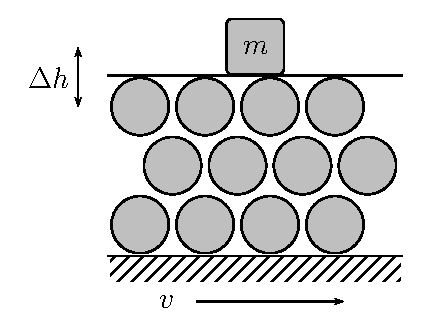
\includegraphics[width=0.4\textwidth]{./figs/comparison2.eps} &
    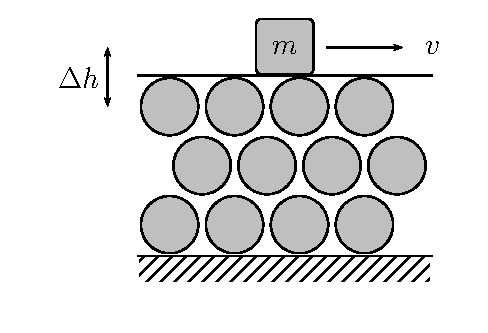
\includegraphics[width=0.46\textwidth]{./figs/comparisonD.eps}\\
    \hspace{1.2cm}(c) & \hspace{1.2cm}(d) \\
    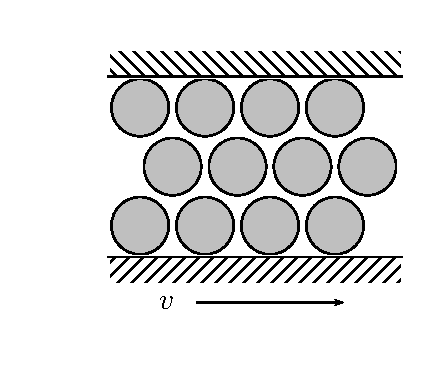
\includegraphics[width=0.4\textwidth]{./figs/comparisonC.eps} &
    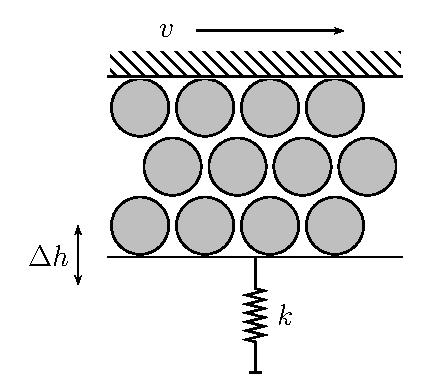
\includegraphics[width=0.4\textwidth]{./figs/comparison3.eps}\\
  \end{tabular}
\caption[Schematics of different types of experimental devices
used to study granular shear flow.]{Schematics of different types of experimental devices
used to study granular shear flow. (a) and (b) represent constant
load devices, where compaction and dilation are allowed. The
difference between (a) and (b) is whether the system is sheared at
the top or from the bottom surface. (c) Constant volume shear
cell. (d) The annular shear cell used in the present study. In the
present experimental device the bottom surface is also allowed to
tilt.} \label{fig:figcomp}
\end{figure}

\clearpage %Thesis
\section{RESULTS}\label{sec:results}
\par Depending on the type of the work then results are presented in a separate section. Sometimes the arrangements for the experiments are also described in this section. And in some cases the section contains also some consideration of the quality of the results, even some discussion and conclusions. It might be reasonable to divide section ``Results'' into several, e.g. ``Experiments'' and ``Results''. Discuss these options with your supervisor.  The thesis also contains some discussion about the future work.
 
\par Define the structure of the thesis according to your requirements. Discuss the structure with you supervisor(s). There can be subsections in each section, and also sub-subsections if needed. Keep in mind that the thesis is an independent presentation of the work done. The presentation is also consistent and logical, everything is carefully considered and presented.  
 %Results
\section{DISCUSSION AND CONCLUSIONS}\label{sec:conslusions}
\par In most cases it is reasonable to present new findings and main results in a separate section. This section also further analyzes observations and results. This section is also the place to include the synthesis of the results, the future possibilities in the research topic or the in the application area. After discussion and consideration one should present the conclusions. This section contains the reasoning for those conclusions. In the next section, in the summary, one just lists the conclusions.
  %Conclusions

%\def\refname{what ever}% to change References title
\addcontentsline{toc}{section}{REFERENCES}%

\appendix
% Uncomment if page number in header
% \fancyhead[LO]{}     %
% \fancyhead[RE]{}%
\section*{APPENDICES}\label{sec:appendices}
\addcontentsline{toc}{section}{APPENDICES}
\renewcommand{\thesubsection}{APPENDIX \arabic{subsection}.}
\subsection*{APPENDIX 1. Results from the experiments}\label{sec:appendix1}
\par Now the Appendix 1 continues on this page. Naturally the previous page is full of text, or if there are large tables etc, then allocate space using the rules for the body of the thesis. Since there is no text ``(continues)'' at the bottom of this page, then the reader knows that this is the last page for Appendix 1.

\clearpage
\pagebreak

\subsection*{APPENDIX 1. Results from the experiments (continued)}
\par Now the Appendix 1 continues on this page. Naturally the previous page is full of text, or if there are large tables etc, then allocate space using the rules for the body of the thesis. Since there is no text ``(continues)'' at the bottom of this page, then the reader knows that this is the last page for Appendix 1.

\bibliography{ref}%
\bibliographystyle{LUTapa}%

\cleardoublepage %

\end{document}
